\chapter{Mining item-centric top-$k$ closed itemsets with \toppi}
\label{chap:toppi}


\minitoc


Given a transactional dataset,
without additional knowledge
it is tempting to search for frequent items associations.
%especially as many mining algorithms have been proposed.
An attempt to apply such algorithms directly raises a question:
how many occurrences make an itemset frequent? A thousand? Ten? One percent?
Indeed, the algorithm needs this threshold to be fixed before starting the computation.
A quick study of the items' individual frequencies may give a first hint of a relevant threshold.
In practice, though, the analyst often does a more iterative guess.
Starting from a high frequency threshold ($10\%$, for example),
she progressively lowers the threshold until she finds interesting results.
This makes the discovery process more and more difficult,
as lowering the frequency threshold yields more and more results
(even with the restriction to closed itemsets).
%For exploration purposes,
Indexing the resulting CIS by item is quite intuitive.
But the analyst would expect such an index to include any item,
% that may show even a small coincidence between transactions.
because she can be interested in any item's association.
This is particularly true at the first encounter with a dataset,
when analysts need to explore easily all its aspects.

Applying itemset mining on millions of transactions therefore raises the following problems:

\begin{itemize}
	\item A single mining attempt should provide results about all items appearing in at least two transactions.
	But, as seen from existing algorithms, this is close to mining {\em all} CIS.

	\item The input dataset is the only knowledge we have,
		hence our parameter(s) should only express the desired quantity of output.

	\item The processing should be parallelized,
		in order to fit in the systems which are usually storing datasets as big as ours.
\end{itemize}

%we present centralized and distributed variants of the algorithm.

These challenges lead us to propose an {\em item-centric} problem statement
and an algorithm to solve it, \toppi.
The present chapter details our contributions :

\begin{itemize}
	\item We formalize item-centric mining,
	and highlight its afferent challenges with an experiment and an example, in Section~\ref{sec:toppi:intro}.

	\item We detail our algorithm, its heuristics and pruning strategies
	in Section~\ref{sec:toppi:algo}.

	\item We show how to leverage additional CPUs or machines for item-centric mining in Section~\ref{sec:toppi:hadoop}.

	\item Section~\ref{sec:toppi:xp} shows example results and evaluates experimentally \toppi.
		We show that it outperforms similar or straightforward solutions,
		and measure its speedup on both our {\em server} and {\em cluster} platforms.

	\item Thanks to the technology transfer to the \datalyse project,
	 we provide industrial feedback on the run-time performance and results quality of \toppi
	 in Section~\ref{sec:toppi:integration}.
\end{itemize}


%We conclude in Section~\ref{sec:toppi:conc}.



\section{Item-centric itemset mining: goal and challenges}
\label{sec:toppi:intro}

We start by further discussing how item-centric mining differs from frequent CIS mining.
Section~\ref{sec:toppi:statement} formalizes \toppi's problem statement.
In Section~\ref{sec:toppi:jclmCoverage} we show experimentally that a frequent itemset mining algorithm like \jlcm
fails to provide results that satisfy our problem statement.
Finally Section~\ref{sec:toppi:tree} gives a first intuition of \toppi's underlying principles,
by detailing a CIS enumeration.
This example allows us to precise the challenges inherent to item-centric itemset mining.


\subsection{Relevant semantics for long-tailed datasets}
\label{sec:toppi:statement}

As the number of transactions increases,
searching iteratively for the right frequency threshold becomes less and less convenient ---
not because of the computation time, but because of the number of results.
In our {\em server} setting,
once the dataset is loaded in memory and using a frequency threshold of \num{32000} (\num{0.01}\%),
it takes less than 2 minutes to extract \num{50464} closed itemsets (CIS)
out of \prodassocreceipt with \jlcm.
But %even with an additional filtering, by imposing a minimal \colorred{confidence UNDEF},
browsing such results set is too cumbersome for the analyst.
Looking back at Figure~\ref{fig:itemFreqDist} (p.\pageref{fig:itemFreqDist})
we also observe that \num{92}\% of the articles are filtered out with this threshold.
In other words, our results show associations between only \num{8}\% of the available articles.
We could include more articles by lowering the frequency threshold,
but this would produce an overwhelming amount of results.
In \prodassocreceipt again, after 4 minutes of computation we can find the
\num{376495} itemsets appearing more than \num{10000} times.
But they only cover \num{13}\% of the articles.
This observation also applies to Web datasets,
which often follow a ``long tail'' distribution~\cite{GoelWSDM10}.

\begin{figure}
	\centering
	\begin{subfigure}[b]{0.48\textwidth}
		\centering
		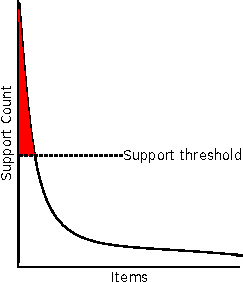
\includegraphics{fig/topPI-vs-classic/freq_distrib_standard.pdf}
		\caption{Frequent Itemset Mining}
	\end{subfigure}
	\hfill
	\begin{subfigure}[b]{0.48\textwidth}
		\centering
		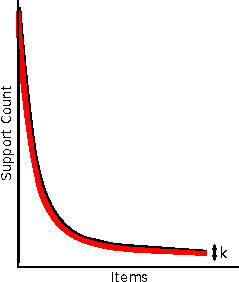
\includegraphics{fig/topPI-vs-classic/freq_distrib_topk.pdf}
		\caption{Our approach, \toppi}
	\end{subfigure}
	\caption{\label{fig:toppiVSclassic}
		Schematic distinction between frequent itemsets mining and \toppi.
		The area in red represent each method's output.
	}
\end{figure}

A common request in the retail industry is
the ability to access a product's sales trends and associations with other products.
This allows managers to obtain feedback on customer behavior
and to propose relevant product bundles.
Whether items are products, categories or segments,
the analyst will spontaneously search for an item she already knows,
discover new items associated to the first one,
continue to one of the new items' associations, and so on.
Hence our item-centric approach and our introduction of a unique parameter:
$k$, the number of itemsets to be returned per item.

Figure~\ref{fig:toppiVSclassic} illustrates our distinction from frequent itemset mining algorithms.
%who tend to generate many itemsets out of the few frequent ones.
\toppi extracts itemsets for all items,
therefore providing the analyst with an overview of the dataset.
As illustrated in the previous paragraph,
this is essential when discovering a transactional dataset.

\toppi is also beneficial to other applications such as query recommendation~\cite{LiRecSys08},
where we usually should give a dozen recommendations related to a requested item.
\toppi ensures the ability to answer recommendation queries, even for rare terms.
We therefore formalize the objective of \toppi as follows:

\begin{definition} Given a dataset ${\cal D}$ and
an integer $k$, \toppi returns, for each item in ${\cal D}$,
the $k$ most frequent closed itemsets containing this item.
\end{definition}

\begin{table}
	\begin{subtable}[b]{0.48\textwidth}
		\centering
		\begin{tabular}{|r|l|l|}
  \hline
  TID   & Transaction \\ \hline
  $t_0$ & $\{0,1,2\}$       \\
  $t_1$ & $\{0,1,2\}$       \\
  $t_2$ & $\{0,1\}$         \\
  $t_3$ & $\{2,3\}$       \\
  $t_4$ & $\{0,3\}$       \\\hline
\end{tabular}

		\caption{\label{tab:toppi:sample:in}Dataset $\cal D$}
	\end{subtable}
	\hfill
	\begin{subtable}[b]{0.48\textwidth}
		\centering
		\begin{tabular}{|c|l|l|}
			\hline
			item   & \multicolumn{2}{c|}{$\mathit{top}(i)$: $P$, $\mathit{support}(P)$} \\
			$i$& $1^{st}$ &$ 2^{nd}$\\
			\hline
			$0$ & $\{0\},4$ & $\{0,1\},3$ \\
			$1$ & $\{0,1\},3$ & $\{0,1,2\},2$ \\
			$2$ & $\{2\},3$ & $\{0,1,2\},2$ \\
			$3$ & $\{3\},2$ & \\\hline
		\end{tabular}
		\caption{\label{tab:toppi:sample:out}Results for $k=2$}
	\end{subtable}
	\caption{Example \toppi input and output}
\end{table}


Table~\ref{tab:toppi:sample:out} shows the solution to this problem applied to the dataset in
Table~\ref{tab:toppi:sample:in}, with $k=2$.
Note that we purposely ignore itemsets that occur only once,
as they do not show a behavioral pattern.
The restriction to closed itemsets avoid redundant results
(as discussed in Sections~\ref{sec:model:mining} and \ref{sec:lcm}).
The number of itemsets returned for each item
may be tuned depending on the application.
If the itemsets are directly presented to an analyst,
$k=10$ can be sufficient, while $k\geq\num{100}$ may be used when those itemsets are analyzed automatically.

\toppi relies on frequency to rank each $k$ itemsets associated with an item.
Another possibility would have been to rank the itemsets associated to an item
by statistical correlation with this item, using for example the $p$-value as a measure.
However, ranking by $p$-value implies a much wider exploration of the itemsets space,
because the strongest correlations are sometimes found with rare itemsets~\cite{MinatoKDD14}.
This also applies to other quality measures, which are not affordable at our target scale.
%Furthermore,
%we show experimentally that \toppi's output is very close to top-$k$ itemsets ranked by $p$-value.
We instead propose, in Section~\ref{sec:quali:pval} (p.\pageref{sec:quali:pval}),
to re-rank \toppi's results according to a finer quality measure.





\subsection{First challenge: the need for a specialized algorithm}
%Emulating item-centric mining with \jlcm or TFP
\label{sec:toppi:jclmCoverage}


We now present and discuss
preliminary experiments showing that we cannot perform item-centric mining with existing algorithms.

The most obvious solution is to use a global top-$k$-frequent CIS miner like TFP~\cite{HanICDM02}
on each projected dataset ${\cal D}[i]$, for each item $i$.
This solution runs out of memory on our datasets.
Even if we let it benefit from one of our optimizations,
it is not as robust as our dedicated algorithm --- this is further discussed in the Section~\ref{sec:toppi:xp:server} of our experiments.


\begin{figure}
	\centering
	\begin{tabular}{cc}
		\begin{subfigure}[b]{0.48\textwidth}
			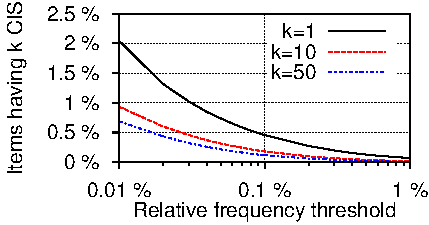
\includegraphics{fig/toppi/classic-vs-topPI/nbTopK-classic-lastfm.pdf}
			\caption{\em LastFM}
		\end{subfigure}
		&
		\begin{subfigure}[b]{0.48\textwidth}
			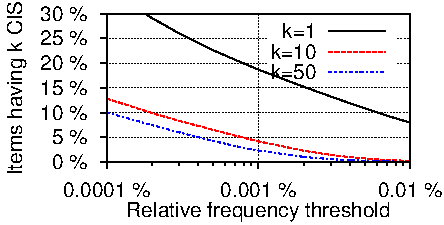
\includegraphics{fig/toppi/classic-vs-topPI/nbTopK-classic-tickets2013.pdf}
			\caption{\prodassocreceipt}
		\end{subfigure}
		\\
		\begin{subfigure}[b]{0.48\textwidth}
			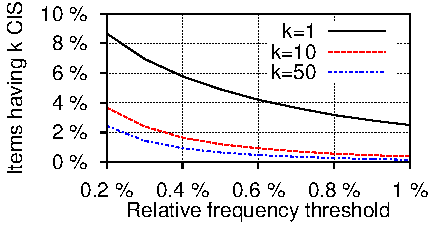
\includegraphics{fig/toppi/classic-vs-topPI/nbTopK-classic-tickets2013-perClient.pdf}
			\caption{\prodassocclient}
		\end{subfigure}
		&
		\hfill
		\begin{minipage}[b]{0.40\linewidth}
			\caption{\label{fig:classicCoverage}
				Proportion of available items appearing in at least $k$ itemsets (for $k \in \{1, 10, 50\}$),
				using frequent CIS mining,
				with respect to the frequency threshold.
			}
		\end{minipage}
		\\
	\end{tabular}
\end{figure}


In this section we present another experiment,
where we simulate item-centric mining with our frequent CIS mining algorithm, \jlcm
(fully presented in Section~\ref{sec:lcm}, p.\pageref{sec:lcm}).
%Given a frequency threshold $\varepsilon$, the algorithm extracts all CIS whose support is above $\varepsilon$.
The top-$k$ CIS of each item can be computed as a post-processing of these results,
thus producing the same output as \toppi.
We evaluate this approach for different frequency thresholds $\varepsilon$ and present the results in Figure~\ref{fig:classicCoverage}.
This post-processing approach does not take the number of desired CIS per item $k$ as a parameter,
so instead we measure for each value of $\varepsilon$ the number of items appearing in at least $k$ CIS, for 3 values of $k$.

Each item is present in at least one CIS,
whose support is equal to the frequency of the item in the dataset.
This CIS, a singleton in most cases, is the only result sufficient for $k=1$.
We already notice that, because of the long-tailed distribution of the data,
it is necessary to reach very low values of $\varepsilon$ to select a large number of items.
In the case of {\em LastFM}, only 2\% of items appear in more than $\num{0.01}\%$ of the transactions.
Furthermore, for the same value of $\varepsilon$, only 1\% of items are included in more than 10 frequent CIS.
But it takes 150 hours of CPU time to extract all CIS at this support threshold:
the algorithm mines over 2 billion CIS, and only $\num{24536}$ items out of 1.2 million appear in these results.

The behavior of this approach on \prodassocreceipt, although slightly better, highlights the same limitations.
Using a frequency threshold of $10^{-5}\%$, mining frequent CIS takes one hour.
This may appear to be a reasonable run-time, but the results are not very useful for the analysts:
the $\num{34151639}$ CIS only contain a minority of the available products,
and 90\% of the items are in less than 10 CIS.
We obtain similar figures over \prodassocclient:
when $\varepsilon = 0.2\%$,
it takes 45 hours of CPU time to obtain $\num{13612569}$ CIS covering less than $10\%$ of the available items.

As this experiment shows, standard CIS mining algorithms are perfectly capable of efficiently enumerating billions of CIS.
The problem is that these itemsets only contain the most frequent items in the dataset, and fail to cover items from the long tail.
Hence, the post-processing approach spends most of the mining time generating an overwhelming amount of CIS which are of no interest to the analyst.
This observation motivated the development of \toppi,
that efficiently computes item-centric CIS using an integrated approach.
We leverage the efficient enumeration principles from LCM,
but use different heuristics and pruning to perform item-centric mining.


\subsection{Second challenge: pruning while garanteeing correctness}
\label{sec:toppi:tree}


\begin{figure}
	\centering
	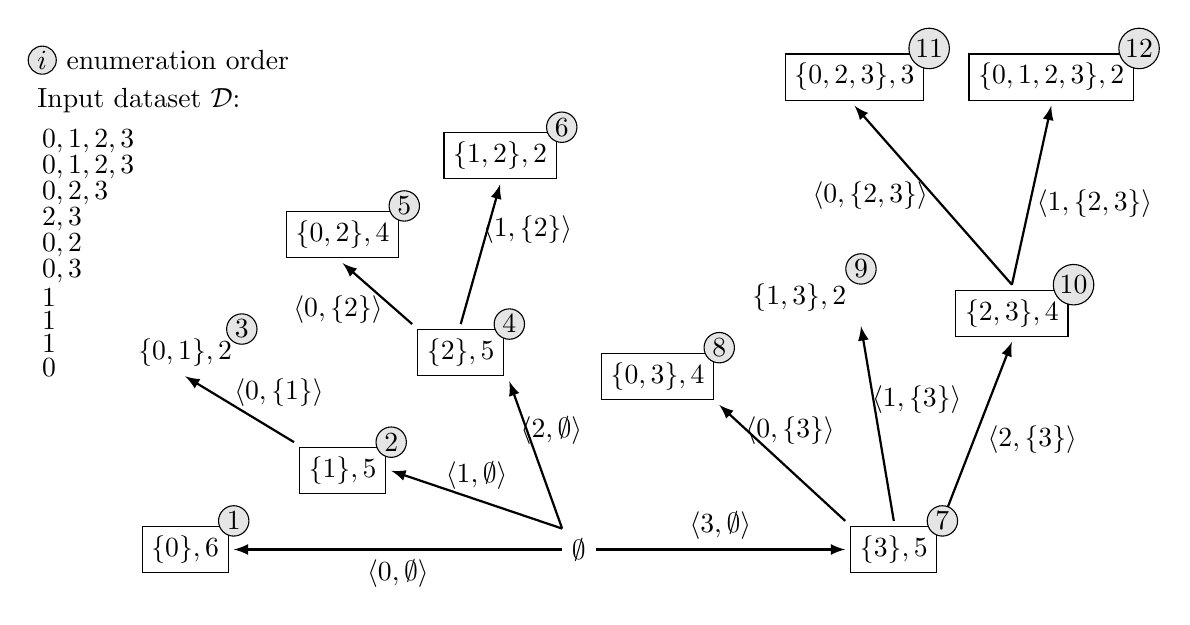
\begin{tikzpicture}[>=latex]%[>=triangle 45]
		\node[inner ysep=1em,anchor=west] (t0) at (-7,5.7) {Input dataset $\cal D$:};
		\node[inner sep=0.5em,anchor=west] (t1) at (t0.south west) {$0, 1, 2, 3$};
		\node[inner sep=0.5em,anchor=west] (t2) at (t1.south west) {$0, 1 , 2, 3$};
		\node[inner sep=0.5em,anchor=west] (t3) at (t2.south west) {$0, 2, 3$};
		\node[inner sep=0.5em,anchor=west] (t4) at (t3.south west) {$2, 3$};
		\node[inner sep=0.5em,anchor=west] (t5) at (t4.south west) {$0, 2$};
		\node[inner sep=0.5em,anchor=west] (t6) at (t5.south west) {$0, 3$};
		\node[inner sep=0.5em,anchor=west] (t7) at (t6.south west) {$1$};
		\node[inner sep=0.5em,anchor=west] (t8) at (t7.south west) {$1$};
		\node[inner sep=0.5em,anchor=west] (t9) at (t8.south west) {$1$};
		\node[inner sep=0.5em,anchor=west] (t10) at (t9.south west) {$0$};

		\node (legenC)[draw,circle,fill=gray!20,inner sep=1pt,anchor=west] at (t0.north west) {$i$};
		\node [right] at (legenC.east) {enumeration order};



		\node (empty) at (0,0) {$\emptyset$};

		\node (0)     [draw,outer sep=2pt] at (-5,0) {$\{0\},6$};
		\node (s0)    [draw,circle,fill=gray!20,inner sep=1pt] at (0.north east) {1};
		\draw [->,thick] (empty.west) -- (0.east) node[below, midway] {$\langle 0, \emptyset\rangle$};

		\node (1)     [draw,outer sep=2pt] at (-3,1) {$\{1\},5$};
		\node (s1)    [draw,circle,fill=gray!20,inner sep=1pt] at (1.north east) {2};
		\draw [->,thick] (empty.north west) --(1.east) node[above, midway] {$\langle 1, \emptyset\rangle$};

		\node (01)     at (-5,2.5) {\st{$\{0,1\},2$}};
		\node (s01)    [draw,circle,fill=gray!20,inner sep=1pt] at (01.north east) {3};
		\draw [->,thick] (1.north west) --(01.south) node[above, midway, xshift=0.5cm, yshift=-0.1cm] {$\langle 0, \{1\}\rangle$};

		\node (2)     [draw,outer sep=2pt] at (-1.5,2.5) {$\{2\},5$};
		\node (s2)    [draw,circle,fill=gray!20,inner sep=1pt] at (2.north east) {4};
		\draw [->,thick] (empty.north west)--(2.south east) node[above, midway, xshift=0.2cm] {$\langle 2, \emptyset\rangle$};

		\node (02)    [draw,outer sep=2pt] at (-3,4) {$\{0,2\},4$};
		\node (s02)   [draw,circle,fill=gray!20,inner sep=1pt] at (02.north east) {5};
		\draw [->,thick] (2.north west)--(02.south) node[below, midway, xshift=-0.5cm, yshift=0.1cm] {$\langle 0, \{2\} \rangle$};

		\node (12)    [draw,outer sep=2pt] at (-1,5) {\st{$\{1,2\},2	$}};
		\node (s12)   [draw,circle,fill=gray!20,inner sep=1pt] at (12.north east) {6};
		\draw [->,thick] (2.north)--(12.south) node[above, midway, xshift=0.6cm] {$\langle 1, \{2\} \rangle$};

		\node (3)     [draw,outer sep=2pt] at (4,0) {$\{3\},5$};
		\draw [->,thick] (empty.east)--(3.west) node[above, midway] {$\langle 3, \emptyset \rangle$};

		\node (03)     [draw,outer sep=2pt] at (1,2.2) {$\{0,3\},4$};
		\node (s03)    [draw,circle,fill=gray!20,inner sep=1pt] at (03.north east) {8};
		\draw [->,thick] (3.north west)--(03.south east) node[above, midway, xshift=0.1cm, yshift=0.1cm] {$\langle 0, \{3\}\rangle$};

		\node (13)     [outer sep=2pt] at (2.8,3.2) {\st{$\{1,3\},2$}};
		\node (s13)    [draw,circle,fill=gray!20,inner sep=1pt] at (13.north east) {9};
		\draw [->,thick] (3.north)--(13.south east) node[above, midway, xshift=0.5cm] {$\langle 1, \{3\}\rangle$};

		\node (23)     [draw,outer sep=2pt] at (5.5,3) {$\{2,3\},4$};
		\node (s23)    [draw,circle,fill=gray!20,inner sep=1pt] at (23.north east) {10};
		\draw [->,thick] (3.north east)--(23.south) node[below, midway, xshift=0.7cm, yshift=0.2cm] {$\langle 2, \{3\} \rangle$};

		\node (s3)    [draw,circle,fill=gray!20,inner sep=1pt] at (3.north east) {7};

		\node (023)     [draw,outer sep=2pt] at (3.5,6) {$\{0,2,3\},3$};
		\node (s023)    [draw,circle,fill=gray!20,inner sep=1pt] at (023.north east) {11};
		\draw [->,thick] (23.north)--(023.south) node[below, midway, xshift=-0.8cm, yshift=0.3cm] {$\langle 0, \{2,3\} \rangle$};

		\node (123)     [draw,outer sep=2pt] at (6,6) {$\{0,1,2,3\},2$};
		\node (s123)    [draw,circle,fill=gray!20,inner sep=1pt] at (123.north east) {12};
		\draw [->,thick] (23.north)--(123.south) node[below, midway, xshift=0.8cm, yshift=0.2cm] {$\langle 1, \{2,3\} \rangle$};

	\end{tikzpicture}
	\caption{\label{fig:expand:example}
		An example dataset and its corresponding CIS enumeration tree in \jlcm.
		Each node is an itemset and its support.
		$\langle i,P\rangle$ denotes the closure extension operation.
		Striked out itemsets are candidates failing the first-parent test (Algorithm~\ref{alg:jlcm}, line~\ref{line:LCM1stparent}, p.\pageref{alg:jlcm}).
	}
\end{figure}


We now discuss how we can optimize and prune \jlcm's enumeration for item-centric mining,
over the example of Figure~\ref{fig:expand:example}, where $k=2$.
In this example we follow the $\mathit{expand}$ function presented in Algorithm~\ref{alg:jlcm}, p.\pageref{alg:jlcm}.
The only modification is that we now assume that the enumerated CIS are progressively kept in a collection of heaps,
denoted $\mathit{top}(i)$ for each item $i$.
Items are already indexed by decreasing frequency.
Candidate extensions of steps \circled{3} and \circled{9} are not collected as they fail the first-parent test
(their closure is $\{0,1,2,3\}$).

In frequent CIS mining algorithms, the frequency threshold allows the program
to lighten the intermediate datasets (${\cal D}_I$) involved in the enumeration.
In \toppi we have an implicit minimum support $\varepsilon$ equal to 2,
because we are not interested in CIS occurring only once.
Though, increasing $\varepsilon$ above 2, when exploring some parts of the CIS space,
could speed up the exploration as in a frequent CIS miner.
This is the goal of the dynamic threshold adjustment proposed in \toppi.
In our example, before step {\scriptsize\circled{4}} we can compute items' supports in ${\cal D}[2]$
--- these supports are re-used in $\mathit{expand}(\emptyset, 2, {\cal D}, \varepsilon)$ ---
and observe that the two most frequent items in ${\cal D}[2]$ are 2 and 0, with respective supports of 5 and 4.
These will yield two CIS of supports 5 and 4 in $\mathit{top}(2)$.
The intuition of dynamic threshold adjustment is that 4 might therefore be used as a frequency threshold in this branch.
It is not possible in this case because a future extension, 1,
does not have its $k$ itemsets at step {\scriptsize\circled{4}}.
This is also the case at step {\scriptsize\circled{7}}.
The dynamic threshold adjustment done in \toppi takes this into account,
in order to ensure its results' correctness.

After step {\scriptsize\circled{8}}, $\mathit{top}(0)$, $\mathit{top}(2)$ and $\mathit{top}(3)$
already contain two CIS, as required, all having a support of 4 or more.
Hence it is tempting to prune the extension $2,\langle\{3\}\rangle$ (step {\tiny\circled{10}}),
as it cannot enhance $\mathit{top}(2)$ nor $\mathit{top}(3)$.
However, at this step,
$\mathit{top}(1)$ only contains a single CIS and 1 is a future extension.
Hence {\tiny\circled{10}} cannot be pruned:
although it yields an useless CIS, one of its extensions leads to a useful one (step {\tiny\circled{12}}).
In this tree we can only prune the recursion towards step {\tiny\circled{11}}.

This example's distribution is unbalanced in order to show \toppi's corner cases with only 4 items;
but in real datasets, with hundreds of thousands of items, such cases regularly occur.
This shows that an item-centric mining algorithm requires rigorous strategies
for both pruning the search space and filtering the datasets.


Rather than exhaustively extracting the most frequent itemsets,
\toppi ensures that all items are covered by the results
and restricts its search space according to the $k$ parameter.
Our datasets' size raises an additional challenge:
the exploration and pruning strategy should remain efficient
when parallelized, in order to handle millions of transactions
in a reasonable amount of time.
%We design an algorithm that restricts the space of itemsets explored
%to keep the execution time within reasonable bounds.










\section{\toppi algorithm}
\label{sec:toppi:algo}

We now present our sequential solution of item-centric CIS mining, the \toppi algorithm.

\begin{paragraph}{Dataset notations reminder}
	$\cal D$ is our input dataset, a collection of transactions.
	Given an itemset $I$, the projected dataset of $I$ is
	${\cal D}[I] = \langle t \in {\cal D} \mid I \subseteq t \rangle$.
	Its reduced dataset is ${\cal D}_I = \langle t \setminus I \mid t \in {\cal D}[I]\rangle$.
	When $I$ is a singleton $\{i\}$, we may omit the braces and write ${\cal D}[i]$ and ${\cal D}_i$.
\end{paragraph}


\subsection{\toppi architecture}
\label{sec:algo:intro}

\begin{figure}
	\centering
	\input{svg/toppi/Architecture.pdf_tex}
	\caption{\label{fig:toppi:arch}
	\toppi's architecture.
	}
\end{figure}

Figure~\ref{fig:toppi:arch} gives an overview of \toppi.
The CIS enumeration at the core of
\toppi follows principles from \jlcm (presented in Section~\ref{sec:lcm}, p.\pageref{sec:lcm}).
In \toppi it is done by a variant of the $\mathit{expand}$ function,
presented in Section~\ref{sec:toppi:expand}.
Similarly to traditional top-$k$ processing approaches~\cite{FaginPODS01},
\toppi relies on heap structures to progressively collect its top-$k$ results,
and outputs them once the execution is complete.
More precisely, \toppi stores traversed itemsets in a \emph{top-$k$ collector} which maintains,
for each item $i\in{\cal I}$, $\mathit{top(i)}$,
a heap of size $k$ containing the current version of the $k$ most frequent CIS containing $i$.
As soon as a CIS and its support is discovered by $\mathit{expand}()$,
it is kept in the top-$k$-collector via the $\mathit{collect}()$ function.
We can query the top-$k$-collector through $\mathit{lowestSupportIn(top(i))}$,
which is the $k^{th}$ support value in $\mathit{top(i)}$, or 2 if $|\mathit{top(i)}|<k$.
%It can be considered as a frequency threshold to enter the top-$k$ of the item $i$.
We mine all the $k$-lists simultaneously to maximize the amortization of each itemset's computation.
Indeed an itemset is a candidate for insertion in the heap of all items it contains.
Moreover, as shown in Chapter~\ref{chap:model},
the analysis is not performed on the live transaction database but on dedicated machines.
Hence we choose to create an itemset database for the associations explorer application.

\toppi introduces an adequate pruning of the solutions space.
For example, we should be able to prune
an itemset $\{a,b,c\}$ once we know it is not a top-$k$ frequent for $a$, $b$ nor $c$.
However, as highlighted in the previous example (Section~\ref{sec:toppi:tree}),
we cannot prune $\{a,b,c\}$ if it precedes interesting CIS in the enumeration.
\toppi's $\mathit{prune}$ function, presented in Section~\ref{sec:toppi:pruning},
tightly cuts the CIS space while ensuring results' completeness.
Section~\ref{sec:toppi:shortcut} how we can simplify its computation with {\em prefix short-cutting}.

The CIS exploration is initiated by the $\mathit{startBranch}$ function,
presented in Section~\ref{sec:toppi:start},
which enumerates itemsets $P$ such that $\mathit{max}(P)=i$.
\toppi does not require the user to define a minimum frequency,
but we observe that the support range in each item's top-$k$ CIS varies by orders of magnitude from an item to another.
Because filtering out less frequent items can speed up the CIS enumeration in some branches,
$\mathit{startBranch}$ implements a {\em dynamic threshold adjustment}:
it tries to find the greatest frequency threshold $\varepsilon$
that garantees our results' completeness in each branch.
$\varepsilon$ defaults to 2, because we are not interested in itemsets occurring once.



\begin{algorithm}
	\caption{\toppi's main function}
	\label{alg:toppi:main}
	\KwData{dataset $\cal D$, integer $k$}
	\KwResult{Output top-$k$ CIS for all items of ${\cal D}$}
	\Begin{
		\ForEach(\tcp*[f]{Collector instantiation}){$i \in {\cal I}$\label{line:initcollectstart}}{
					\textbf{initialize} $\mathit{top(i)}$, heap of max size $k$\label{line:initcollectend}
		}
		%$\emptyset_{closed} \gets \bigcap_{t \in {\cal D}}\ t$ \\
		%$\mathit{collect(\emptyset_{closed},|{\cal D}|})$\\

		\ForEach(\tcp*[f]{In increasing item order}){$i \in {\cal I}$\label{line:topLCMstarters}}{
			$startBranch(i,{\cal D},k)$\label{line:startBranchInvoc}
		}
	}
\end{algorithm}


The main program, presented in Algorithm~\ref{alg:toppi:main},
initializes the collector in lines~\ref{line:initcollectstart} and \ref{line:initcollectend}.
Then it invokes, for each item $i$,
$\mathit{startBranch(i, {\cal D}, k)}$.
In our examples, as in \toppi, items are represented by integers.
While loading $\cal D$, \toppi indexes items by decreasing frequency,
hence 0 is the most frequent item.
Items are enumerated in their natural order in line~\ref{line:topLCMstarters},
thus items of greatest support are considered first.








\subsection{CIS enumeration in \toppi}
\label{sec:toppi:expand}

\begin{algorithm}
  \caption{\toppi's CIS exploration function}
	\label{alg:toppi:expand}
	\SetKwProg{myproc}{Function}{}{}
	\myproc{$\mathit{expand}(I,e,{\cal D}_I,\varepsilon$)}{
		\KwData{CIS $I$, extension item $e$, reduced dataset ${\cal D}_I$, frequency threshold $\varepsilon$}
		\KwResult{If $\langle e, I\rangle$ is a relevant closure extension, collects CIS containing $\{e\}\cup I$ and items smaller than $e$}
		\Begin{
			$J \gets \mathit{closure}(\{e\}\cup I)$  \label{line:closure}\\
			\If{$\mathit{max}(J \setminus I) = e$\label{line:fptest}}{
      	$\mathit{collect}(J,\mathit{support}_{\cal D}(J), \mathit{true})$ \tcp*[f]{Update top-k-collector} \label{line:collect} \\
				\ForEach(\tcp*[f]{In increasing item order}){$i < e \mid \mathit{support}_{{\cal D}_J}[i] \geq \varepsilon$\label{line:enumExtensions}}{
          \If(\tcp*[f]{Additional pruning}){$\neg\mathit{prune}(J,i,{\cal D}_J,\varepsilon)$\label{line:pruneinsert}}{
            $\mathit{expand}(J,i,{\cal D}_J,\varepsilon)$\label{line:recursivecall}
          }
				}
			}
		}
  }
\end{algorithm}


\toppi traverses the CIS space with the $\mathit{expand}$ function,
detailed in Algorithm~\ref{alg:toppi:expand}.
$\mathit{expand}$ performs a depth-first exploration of the CIS tree,
and backtracks when no frequent extension items remain in ${\cal D}_J$ (line~\ref{line:enumExtensions}).
Additionally, in line~\ref{line:pruneinsert}
the $\mathit{prune}$ function (presented in Section~\ref{sec:toppi:pruning})
determines if each recursive call may enhance results held in the top-$k$-collector,
or if it can be avoided.

Upon validating a closure extension $J$,
\toppi updates $\mathit{top(i)}$, $\forall\;i\in J$,
via the $\mathit{collect}$ function (line~\ref{line:collect}).
The support computation exploits the fact that $\mathit{support}_{\cal D}(J) = \mathit{support}_{{\cal D}_I}(e)$,
because $J = \mathit{closure}(\{e\}\cup I)$.
The last parameter of $\mathit{collect}$ is set to \verb|true| to point out that $J$ is a closed itemset
(we show in Section~\ref{sec:toppi:start} that it is not always the case).

%If, for all items to be considered as extensions during the recursive call of line~\ref{line:recursivecall},
%the top-$k$ collector already contains $k$ CIS, all having a support greater than $\mathit{support_{{\cal D}_J}(j)}$,
%then we can safely abort the closure extensions of $\{j\}\cup J$,
%because these extensions will not have a sufficient support to enter the collector.

When enumerating items in line~\ref{line:enumExtensions},
\toppi relies on the items' indexing by decreasing frequency.
As extensions are only done with smaller items this ensures that, for any item $i\in{\cal I}$,
the first CIS containing $i$ enumerated by \toppi combine $i$ with some of the most frequent items.
This heuristic increases their probability of having a high support,
and overall raises the support of itemsets in the top-$k$-collector.

For clarity, the algorithms presented in this chapter do not show the complete implementation of datasets
and their attached structures.
Since the instantiation of projected datasets is the major CPU time consumer,
these are extensively re-used in \toppi:

\begin{itemize}
	\item As our algorithms regularly perform projections on singleton items,
	the input dataset $\cal D$ and reduced datasets ${\cal D}_I$ hold occurrences lists.
	These are indexes providing instantly ${\cal D}[j]$ or ${\cal D}_I[j]$ for any item $j$.
	Those projected datasets are therefore accessed as views over ${\cal D}$ or ${\cal D}_I$, respectively,
	a technique called ``occurrence deliver'' in LCM~\cite{UnoFIMI03}.

	\item In \toppi, as in \jlcm, computing $\mathit{closure(\{e\}\cup I)}$ is done by counting
	items' frequency in ${\cal D}_I[e]$.
	Any item having a 100\% frequency belongs to $J = \mathit{closure(\{e\}\cup I)}$ (Algorithm~\ref{alg:toppi:expand}, line~\ref{line:closure}).
	The resulting item frequency counters are re-used when instantiating the reduced dataset ${\cal D}_J$
	or the set of potential extensions items (Algorithm~\ref{alg:toppi:expand}, line~\ref{line:enumExtensions}).
\end{itemize}




\subsection{Pruning the CIS space}
\label{sec:toppi:pruning}

\begin{algorithm}[t]
	\caption{\toppi's pruning function}
	\label{alg:topk}
	\SetKwProg{myproc}{Function}{}{}
	\myproc{$\mathit{prune(I,e,D_I,\varepsilon)}$}{
	  	\KwData{itemset $I$, extension item $e$, reduced dataset $D_I$, minimum support threshold $\varepsilon$}
	  	\KwResult{\texttt{true} if $\mathit{expand(I,e,{\cal D}_I,\varepsilon)}$ will not provide new results to the top-$k$-collector, \texttt{false} otherwise}
		\Begin{
			\If(\tcp*[f]{Case~\ref{toppi:cq:e}\label{line:extension:start}}){$\mathit{support_{{\cal D}_I}(\{e\})) \geq lowestSupportIn(top(e))}$}{
				\KwRet{\texttt{false}}\label{line:extension:end}
			}
			\ForEach(\tcp*[f]{Case~\ref{toppi:cq:P}\label{line:current:start}}){$i \in I$}{
				\If(\label{line:current:test}){$\mathit{support_{{\cal D}_I}(\{e\})) \geq lowestSupportIn(top(i))}$}{
					\KwRet{\texttt{false}}\label{line:current:end}
				}
			}
			\ForEach(\tcp*[f]{Case~\ref{toppi:cq:others}\label{line:future:start}}){$i < e \mid \mathit{support}_{{\cal D}_I}[i] \geq \varepsilon$}{
				$\mathit{bound} \gets \mathit{min(support_{{\cal D}_I}(\{e\}),support_{{\cal D}_I}(\{i\}))}$\label{line:bound}\\
				\If(){$\mathit{bound \geq lowestSupportIn(top(i))} $\label{line:boundcheckfuture}}{
					%$J \gets \bigcap_{t \in D_P[\{j\}]}t$\label{eq:topkpptest:start}\tcp*[f]{ie. $J \gets \mathit{closure}(\{j\} \cup P)$}\\
					%\If{$\mathit{max(J)} \leq e$\label{eq:topkpptest:end}}{
						\KwRet{\texttt{false}}\label{line:future:end}
					%}
				}
			}
			$\mathit{bound}_\mathit{min}(I) \gets \mathit{min}(\mathit{bound}, \mathit{bound}_\mathit{min}(I))$ \\
			\KwRet{\texttt{true}}
		}
	}
\end{algorithm}


As shown in the example of Section~\ref{sec:toppi:tree},
\toppi cannot prune a sub-tree rooted at $I$ by observing $I$ alone.
We also have to consider itemsets that could be enumerated from $I$ through first-parent closure extensions.
This is done by the $\mathit{prune}$ function presented in Algorithm~\ref{alg:topk}.
It queries the collector to determine whether $\mathit{expand}(I,e,{\cal D}_I,\varepsilon)$
and its recursions may impact the top-$k$ results of an item.
If it is not the case then $\mathit{prune}$ returns \verb|true|,
thus pruning the sub-tree rooted at $\mathit{closure}(\{e\} \cup I)$.

The anti-monotonicity property~\cite{AgrawalVLDB94} ensures that
the support of all CIS enumerated from the closure extension $\langle e, I\rangle$
is smaller than $\mathit{support_{{\cal D}_I}(\{e\})}$.
It also follows from Property~\ref{prop:starters} (p.\pageref{prop:starters}) that the only items
potentially impacted by $\langle e, I\rangle$ are:

\begin{enumerate}
  \item \label{toppi:cq:e} $e$, the extension item;
  \item \label{toppi:cq:P} the items of the extended CIS, $I$;
  \item \label{toppi:cq:others} potentially any item inferior to $e$, to be added by closure or recursive extensions.
\end{enumerate}

The two first cases, considered in lines~\ref{line:extension:start} and \ref{line:current:start},
check $\mathit{top(e)}$ and $\mathit{top(i)}, \forall i \in I$.
Smaller items, which may be included in future extensions of $\{e\}\cup I$,
are considered in lines~\ref{line:future:start}--\ref{line:future:end}.
It is not possible to know the exact support of these CIS, as they are not yet explored.
However we can compute, as in line~\ref{line:bound},
an upper bound such that $\mathit{bound} \geq \mathit{support}(\mathit{closure}(\{i, e\}\cup I))$.
If this bound is smaller than $\mathit{lowestSupportIn(top}(i))$,
then extending $\{e\}\cup I$ with $i$ cannot provide a new CIS to $\mathit{top}(i)$.
Otherwise, as tested in line~\ref{line:boundcheckfuture},
we should let the exploration deepen by returning \verb|false|.
If this test fails for all items $i$,
then it is safe to prune because all $\mathit{top}(i)$ already contain $k$ itemsets of greater support.

The inequalities of lines~\ref{line:extension:start}, \ref{line:current:test} and \ref{line:boundcheckfuture}
are not strict to ensure that no partial itemset
(inserted by the $\mathit{startBranch}$ function, see Section~\ref{sec:toppi:start})
remains at the end of the exploration.
We also remark that the loop of lines \ref{line:future:start}--\ref{line:future:end}
may iterate on up to $|{\cal I}|$ items, and thus may take a significant amount of time to complete.
Hence our implementation of the $\mathit{prune}$ function includes an important optimization.

\subsection{Fast pruning with prefix short-cutting}
\label{sec:toppi:shortcut}

We can leverage the fact that \toppi enumerates extensions by increasing item order.
Let $e$ and $f$ be two items successively enumerated as extensions of a CIS $P$
(Algorithm~\ref{alg:toppi:expand} line~\ref{line:enumExtensions}).
As $e<f$, in the execution of $\mathit{prune}(I,f,{\cal D}_I,\varepsilon)$
the loop of lines \ref{line:future:start}--\ref{line:future:end}
can be divided into:
\begin{itemize}
	\item iterations on items $i \leq e \wedge i \not\in P$,
	\item and the last iteration where $i=f$.
\end{itemize}

We observe that the first iterations were also performed by $\mathit{prune}(I,e,{\cal D}_I,\varepsilon)$,
which can therefore be considered as a prefix of the execution of $\mathit{prune}(I,f,{\cal D}_I,\varepsilon)$.

To take full advantage of this property,
\toppi stores the smallest $\mathit{bound}$ (computed line~\ref{line:bound}) such that
$\mathit{prune}(I, \ast, D_I, \varepsilon)$ returned \verb|true|,
denoted $\mathit{bound}_\mathit{min}(I)$.
This represents the lowest known bound on the support required to enter
$\mathit{top}(i)$, for items $i \in {\cal D}_I$
ever enumerated by line~\ref{line:future:start}.
When evaluating a new extension $f$ by invoking $\mathit{prune}(I,f,{\cal D}_I,\varepsilon)$,
if $\mathit{support}_{{\cal D}_I}(f) \leq \mathit{bound}_\mathit{min}(I)$
then $f$ cannot satisfy any test of lines~\ref{line:current:test} and \ref{line:boundcheckfuture}.
In this case it is safe to skip the loop of lines \ref{line:current:start}--\ref{line:current:end},
and more importantly the prefix of the loop of lines \ref{line:future:start}--\ref{line:future:end},
therefore reducing this latter loop to a single iteration.
As items are sorted by decreasing frequency,
this simplification happens very frequently.

Thanks to prefix short-cutting,
most evaluations of the pruning function are reduced to a few invocations of $\mathit{lowestSupportIn(top(i))}$.
This allows \toppi to guide the itemsets exploration with a negligible overhead.



\subsection{Filtering intermediate datasets with dynamic threshold adjustment}
\label{sec:toppi:start}

If we initiate each CIS exploration branch by invoking $\mathit{expand(\emptyset, i, {\cal D}, 2)}, \forall i \in {\cal I}$,
then $\mathit{prune}$ would be inefficient during the $k$ first recursions
--- that is, until $\mathit{top}(i)$ contains $k$ CIS.
For frequent items, which yield the biggest projected datasets,
letting the exploration deepen with a negligible frequency threshold is particularly expensive.
It is also crucial to diminish the size of the dataset as often as possible,
by filtering out less frequent items that do not contribute to our results.
Hence we propose the dynamic threshold adjustment technique,
to filter projected datasets when possible and avoid the cold start situation.
It is implemented by the $\mathit{startBranch}$ function, presented in Algorithm~\ref{alg:toppi:start}.

\begin{algorithm}
	\caption{\toppi's CIS enumeration branch preparation}
	\label{alg:toppi:start}
  \SetKwProg{myproc}{Function}{}{}
  \myproc{$\mathit{startBranch(i,{\cal D}, k)}$}{
    \KwData{root item $i$, dataset $\cal D$, integer $k$}
	  \KwResult{Enumerates CIS $I$ such that $\mathit{max}(I)=i$}
	  \Begin{
			\ForEach(\tcp*[f]{Pre-filling}){$j\in \mathit{topDistinctSupports}({\cal D}[i], k) \mid i \neq j$\label{line:topitemplaceholders}}{
				$\mathit{collect}(\{i, j\}, \mathit{support}_{{\cal D}[i]}(j), \mathit{false})$\label{line:placeholders}\\
			}
			$\varepsilon_i \gets \mathit{min}_{j \leq i}(\mathit{lowestSupportIn(top(j)))}$\label{line:raiseepsilon}\tcp*[f]{Dynamic th. adjustment}\\
			$\mathit{expand}(\emptyset, i, {\cal D}, \varepsilon_i)$\label{line:expandsingleton}\\
		}
  }
\end{algorithm}


Given a CIS $\{i\}$ and an extension item $e < i$,
computing $Q=\mathit{closure}(\{e\} \cup \{i\})$ is a costly operation
that requires counting items in ${\cal D}_{\{i\}}[e]$.
%However $\mathit{support}(Q)$ can be inferred along the creation of ${\cal D}_{\{i\}}$.
However we observe that $\mathit{support}(Q) = \mathit{support}_{\cal D}(\{e\} \cup \{i\}) = \mathit{support}_{{\cal D}[i]}(e)$,
and the latter value is computed by the items counting
preceding the instantiation of ${\cal D}_{i}$.
Therefore, when starting the branch of the enumeration tree rooted at $i$,
we can already know the supports of some of the upcoming extensions.

The function $\mathit{topDistinctSupports}$ counts items' frequencies in ${\cal D}[i]$ ---
resulting counts are re-used in $\mathit{expand}$ for the instantiation of ${\cal D}_{i}$.
Then, in lines~\ref{line:topitemplaceholders}--\ref{line:placeholders},
\toppi considers items $j$ whose support in ${\cal D}[i]$ is one of the $k$ greatest,
and stores the partial itemset $\{i,j\}$ in the top-$k$ collector (this usually includes $\{i\}$ alone).
We call these itemsets partial because their closure has not been evaluated yet,
so the top-$k$ collector marks them with a dedicated flag:
the third argument of $\mathit{collect}$ is \verb|false| (line~\ref{line:placeholders}).
Later in the exploration,
these partial itemsets are either ejected from $\mathit{top(i)}$ by more frequent CIS,
or replaced by their closure upon its computation (Algorithm~\ref{alg:toppi:expand}, line~\ref{line:collect}).
Thus $\mathit{top(i)}$ contains $k$ itemsets at the end of the loop of lines ~\ref{line:topitemplaceholders}--\ref{line:placeholders}.

The CIS recursively generated by the $\mathit{expand}$ invocation of line~\ref{line:expandsingleton}
may only contain items lower than $i$.
Therefore the smallest $\mathit{lowestSupportIn(top(j))}, \forall j \leq i$,
can be used as a frequency threshold in this branch.
\toppi computes this value, $\varepsilon_i$, on line~\ref{line:raiseepsilon},
in order to filter the biggest projected datasets as a frequent CIS miner would.
This combines particularly well with the frequency-based iteration order,
because $\mathit{lowestSupportIn(top(i))}$ is relatively high for more frequent items.

Note that two partial itemsets $\{i,j\}$ and $\{i,l\}$ of equal support
may in fact have the same closure $\{i,j,l\}$.
Inserting both into $\mathit{top(i)}$ could lead to an overestimation of the frequency threshold,
which would let the enumeration miss legitimate top-$k$ CIS of $i$.
To avoid this, \toppi only selects partial itemsets with {\em distinct} supports.















\section{Scaling \toppi}
\label{sec:toppi:hadoop}

In Section~\ref{sec:toppi:algo} we presented a sequential version of \toppi.
We now describe how \toppi can be deployed on parallel and distributed processing platforms
to process large scale datasets.
The goal is to divide the mining process into independent sub-tasks executed on workers while
ensuring the output completeness, avoiding redundant computation, and maintaining pruning performance.
We first focus on shared-memory parallel architectures in Section~\ref{sec:toppi:multithread}.
Then we consider the case of distributed systems in Section~\ref{sec:toppi:distributed},
and present its implementation over the MapReduce framework~\cite{DeanOSDI04}.
We finally discuss the problem of transactions repartition in a distributed environment in Section~\ref{sec:subdatasets}.

\subsection{Shared-memory parallel systems}
\label{sec:toppi:multithread}

Thanks to our optimizations,
\toppi spends most of its execution time enumerating CIS.
Négrevergne {\em et al.} proposed PLCM, a parallel version of LCM~\cite{NegrevergneHPCS10},
that speeds up significantly this task on multi-core systems.
PLCM dispatches each exploration branch among the available cores.
In a similar fashion,
\toppi instantiates multiple threads and dispatches $\mathit{startBranch}$ invocations.
The collector is shared by all threads, but this does not cause any congestion
because most accesses are read operations from the $\mathit{prune}$ function.

However this could interfere with the dynamic threshold computation, presented in Section~\ref{sec:toppi:start},
because raising the threshold in Algorithm~\ref{alg:toppi:start}, line~\ref{line:raiseepsilon}
requires the top-$k$ of lower items to provide high lower-bounds.
This could also impact the verifications performed by the pruning function
in Algorithm~\ref{alg:topk}, line~\ref{line:future:start}.
For these reasons, we divide  $\mathit{startBranch}$ in two before line~\ref{line:raiseepsilon},
and use a producer-consumer structure to ensure that
the $\varepsilon_i$ computation (Algorithm~\ref{alg:toppi:start}, line~\ref{line:raiseepsilon})
can only be executed for an item $i$ once all items lower than $i$ are done with the top-$k$ collector pre-filling
(Algorithm~\ref{alg:toppi:start}, lines~\ref{line:topitemplaceholders}-\ref{line:placeholders}).
As we experiment in Section~\ref{sec:toppi:xp:hadoop}, this design achieves excellent scalability.




\subsection{Distributed systems and Hadoop implementation}
\label{sec:toppi:distributed}

\begin{figure*}[tb]
	\centering
	\begin{scriptsize}
	\def\svgwidth{\linewidth}
	\input{svg/hadoop.pdf_tex}
	\end{scriptsize}
	\caption{\label{fig:toppihadoop}Hadoop implementation of \toppi}
\end{figure*}

In a distributed setting, we dispatch $\mathit{startBranch}$ invocations among workers.
Figure~\ref{fig:toppihadoop} gives an overview of our solution,
when implemented over the Hadoop framework.
We start by detailing how the CIS exploration is distributed,
then discuss how we dispatch the top-$k$ collector
to ensure its completeness while maintaining its pruning power.
This latter aspect accounts for the separation of item-centric mining in two phases.

\begin{paragraph}{Partitioning the CIS enumeration tree}
	Each worker is assigned a partition of items $G \subseteq {\cal I}$,
	which will be referred to as its {\em group} of items.
	A worker restricts its exploration to the branches starting with an element of $G$
	(Algorithm~\ref{alg:toppi:main}, line~\ref{line:topLCMstarters}, p.\pageref{alg:toppi:main}).
	Following the example of Table~\ref{tab:toppi:ex},
	a worker that is assigned the partition $G=\{0,2\}$ collects the itemsets $\{0\}$,$\{2\}$ and $\{0,1,2\}$.
	It follows from Property~\ref{prop:starters} (p.\pageref{prop:starters})
	that each worker therefore generates a distinct set of itemsets,
	without overlap nor need for a synchronization among them.

	Another benefit of this dispatching is that
	a worker only needs the transactions of ${\cal D}$ that contain items of its partition $G$.
	We call this set of transactions the sub-dataset of the group $G$, denoted ${\cal D}[G]$.
	Our choice to send ${\cal D}$ via the distributed cache for these projections
	(jobs \circled{2} and \circled{3} of Figure~\ref{fig:toppihadoop})
	relies on implementation considerations discussed in Section~\ref{sec:subdatasets}.
	Items are indexed by decreasing frequency in a single MapReduce job
	(Figure~\ref{fig:toppihadoop}, job \circled{1}).
	Then, items are assigned to groups in a round robin fashion.
	This ensures that the most frequent items,
	which form the largest sub-datasets,
	are assigned to different groups.
	This balances the load of workers.

	Note that the CIS enumeration can be parallelized in a worker,
	as presented in the previous section.
	Using all CPUs of a single machine to mine a single sub-dataset ${\cal D}[G]$
	provides an excellent speedup and
	amortizes both the memory consumed by ${\cal D}[G]$
	and the disk/network cost of its instantiation.
\end{paragraph}


\begin{paragraph}{Partitioning the collector}
	Our partitioning of the enumeration tree introduces the drawback that
	the top-$k$ CIS of an item may be generated by any worker,
	without the possibility of predicting which ones.
	A naive solution would make each worker compute a local top-$k$ for all items,
	then merge all local top-$k$ into the exact top-$k$.
	This would require enumerating up to $k\times|{\cal I}|$ CIS per worker,
	thus exploring a much larger fraction of the CIS space than the centralized \toppi
	and significantly limit the scalability.

	Instead, we rely on the following idea:
	if the worker responsible for a group $G$ collects only $\mathit{top(i)}, \forall i \in G$,
	overall we would miss some results, but only a few.
	Indeed, as for $i \in \cal I$ a worker generates CIS combining $i$
	with smaller items of the dataset (\textit{i.e.} more frequent items, thanks to the pre-processing),
	those are likely to have high support.
	But a few CIS in the actual $\mathit{top}(i)$ may be produced by another group's worker.
\end{paragraph}

\begin{table}[tb]
	\centering
	\begin{tabular}{|r|l|l|}
  \hline
  TID   & Transaction \\ \hline
  $t_0$ & $\{0,1,2\}$       \\
  $t_1$ & $\{0,1,2\}$       \\
  $t_2$ & $\{0,1\}$         \\
  $t_3$ & $\{2,3\}$       \\
  $t_4$ & $\{0,3\}$       \\\hline
\end{tabular}

	\caption{\label{tab:toppi:ex}Sample dataset $\cal D$}
\end{table}

\begin{table}[tb]
	\centering
	\begin{tabular}{|c|c|c|c|}
		\hline
		Partition      & Partial top-$k$ (phase 1) & Bounds & Complement top-$k$ (phase 2)\\ \hline
		$G_0$     & $\mathit{top}(0)\rightarrow\{0\}, 4 ; \{0, 1, 2\}, 2$ & $0\rightarrow2$ & $\mathit{top}(1)\rightarrow\{0,1,2\}, 2$ \\
		$\{0,2\}$ & $\mathit{top}(2)\rightarrow\{2\}, 3 ; \{0, 1, 2\}, 2$ & $2\rightarrow2$ & $\mathit{top}(3)\rightarrow\emptyset$        \\ \hline
		$G_1$     & $\mathit{top}(1)\rightarrow\{0,1\}, 3$                & $1\rightarrow0$     & $\mathit{top}(0)\rightarrow\{0,1\}, 3$ \\
		$\{1,3\}$ & $\mathit{top}(3)\rightarrow\{3\}, 2$                  &  $3\rightarrow0$  & $\mathit{top}(2)\rightarrow\emptyset$       \\ \hline
	\end{tabular}
	\caption{\label{tab:toppi:phases}
		2-phase mining over the sample database (Table~\ref{tab:toppi:ex})
		with 2 workers, $k=2$.
	}
\end{table}



Consequently, we run distributed \toppi as a two-phase mining process.
The CIS enumeration is distributed identically in both phases.
We illustrate this process with the example in Table~\ref{tab:toppi:phases}.
In the first phase (Figure~\ref{fig:toppihadoop}, job \circled{2}),
the worker  only collects itemsets for items in $G$ (as described by the previous paragraph).
This is done by restricting the iterated set
at line~\ref{line:future:start} in Algorithm~\ref{alg:topk}.
This phase produces a first, partial version of each item's top-$k$.
It also writes a side output file
which lists $lowestSupportIn(top(i)), \forall i \in \cal I$,
denoted ``Bounds'' in Table~\ref{tab:toppi:phases}
In the second phase (Figure~\ref{fig:toppihadoop}, job \circled{3}),
this list is shared and loaded by each worker,
allowing them to pre-fill their local top-$k$ collector
as if it benefited from the global results of the first phase.
This, in turn, allows the computation of relatively high dynamic thresholds.
Each worker only collects itemsets for items $i \not\in G$ to generate the complement top-$k$.
In this case, the insertion test (line~\ref{line:boundcheckfuture}, Algorithm~\ref{alg:topk})
is ``$i \not\in G$ and $\mathit{bound} \geq \mathit{lowestSupportIn(top(i))}$''.
A final MapReduce job is executed to merge each item's partial top-$k$ and complement top-$k$
(Figure~\ref{fig:toppihadoop}, job \circled{4}).


\begin{paragraph}{}
	As we show in Section~\ref{sec:toppi:xp:hadoop}, in practice this two-phase process is scalable.
	The CIS enumeration is always well divided among workers.
	%and the first phase of mining completely splits the collection among groups,
	%without any impact on the accuracy of pruning.
	We showed theoretically that the second phase is the exact complement of phase one (which prunes too much)
	to overall achieve the same task as the centralized version.
	In practice, the collectors' pre-filling in the second phase allows each worker to benefit
	from the others' work in the first phase,
 	therefore mining is much shorter and accurately targeted to complete the results of phase one.
\end{paragraph}



\subsection{Creating sub-datasets in a distributed environment}
\label{sec:subdatasets}

\begin{figure}
	\centering
	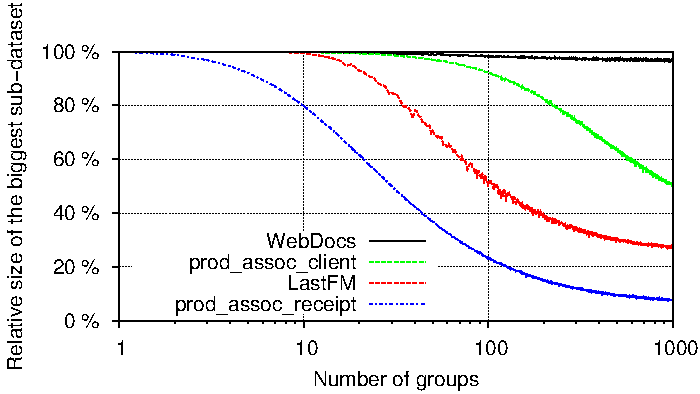
\includegraphics{fig/toppi/G0size/relativeSize.pdf}
	\caption{\label{fig:g0size}Size of the biggest sub-dataset
		relatively to the original dataset's size,
		with respect to the number of groups}
\end{figure}

In a distributed environment,
we partition the items set ${\cal I}$ in item groups $G$ and assign each group to a worker.
This worker needs to load in memory the sub-dataset of $G$,
denoted ${\cal D}[G] = \langle t \in {\cal D} \mid t \cap G \neq \emptyset \rangle$.
As most transactions contain items belonging to different groups,
this does not result in a partition of ${\cal D}$.
We now study how transactions are distributed in the cluster,
and motivate our implementation choices.

Figure~\ref{fig:g0size} shows how the size of the biggest sub-dataset
evolves with respect to the number of groups.
The biggest sub-dataset is the first one,
because it includes the most frequent item, after our re-indexing by decreasing frequency.
We firstly observe that the result is not consistent among datasets.
In the worst case, {\em WebDocs}, the biggest sub-dataset is always almost equal to the complete one,
even when the corresponding worker has to explore a thousand times smaller CIS space.
The length of transactions in {\em WebDocs} accounts for this originality:
its transactions contain 177 items, on average.
But even in the best case
(\prodassocreceipt, in which transactions are much shorter),
when $\cal I$ is divided in 100 partitions this sub-dataset weights much more than 1\% of the original one.
We obtain similar results for the other sub-datasets,
hence the total size of sub-datasets increases in some cases linearly with the number of groups,
as shown by Figure~\ref{fig:gAllSize}.

\begin{figure}
	\centering
	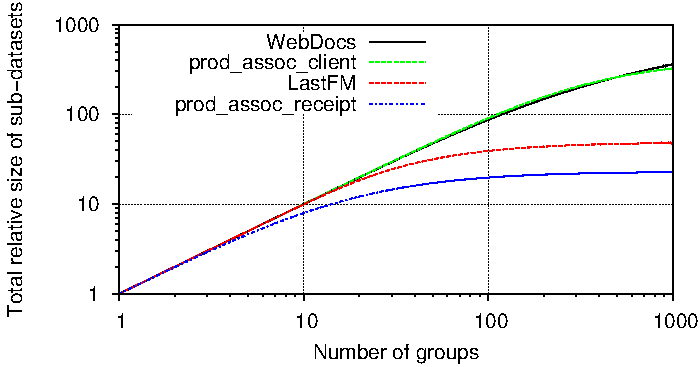
\includegraphics{fig/toppi/G_all_size/relativeSize-total.pdf}
	\caption{\label{fig:gAllSize}Total size of sub-datasets
		relatively to the original dataset's size,
		with respect to the number of groups}
\end{figure}

These measures show that the distributed variant of \toppi is duplicating a non-negligible amount of data.
Indeed the first priority of this version is to distribute and balance the CPU load.
This was motivated by the {\em WebDocs} dataset,
with which \toppi takes more than 9 hours to terminate, even for $k=10$.
As shown by our experiments,
our single server can mine the other datasets in minutes.

Ideally, in order to minimize this data duplication,
we should create as many groups as the number of workers available in the cluster.
However, in our setting a dataset like \prodassocreceipt exhausts workers' memory
if we only create 4 groups (one for each worker of the production cluster).
According to Figure~\ref{fig:g0size}, we can fit sub-datasets in memory by setting the number of groups to 100,
making each machine analyze sequentially 20 different sub-datasets.
But, according to Figure~\ref{fig:gAllSize},
in this case the cluster have to generate 500GB of sub-datasets.

This raises a new question: what is the most effective way to instantiate sub-datasets?
Using the Hadoop framework 3 methods are possible :
\begin{enumerate}
	\item Use a MapReduce job over ${\cal D}$, where for each transaction $t$ the
	\verb|map| function writes a tuple
	$\langle t, gid\rangle, \forall gid \in \{\mathit{group}(i) \mid i \in t\}$.
	Hence each \verb|reduce| function has an instance of $D[G]$ as input.
	This is close to the method adopted by PFP~\cite{LiRecSys08}.
	While it is intuitive, in practice it outputs much data in MapReduce's shuffle'n'sort phase,
	which is highly unusual for a MapReduce job.
 	Such jobs often require a particular tuning of the system.

	\item
	Copy ${\cal D}$ in the distributed cache, such that each worker machine holds a complete copy on its hard drive.
	Then, each task has a to instantiate its sub-dataset by scanning this local copy.
	Although this complete scan is not negligible when the dataset's size is over a gigabyte,
	this method is the fastest in terms of network transfers
	(especially with two-phases mining).

	\item Use the HDFS API to scan ${\cal D}$ at the beginning of each mining task.
	This is the less space consuming for workers but incurs much network traffic,
	especially if more than one mining task is running on a single machine.
\end{enumerate}

Preliminary experiments on {\em LastFM} and {\em WebDocs} show that these methods
are roughly as fast as each other,
but also suggest that such results may be highly platform-dependant.
The projection via the distributed cache has been chosen as it is the most robust
(it does not require Hadoop tuning) and 5 to 50\% faster.




















\section{Evaluation}
\label{sec:toppi:xp}

We now assess experimentally that \toppi outperforms naive or existing solutions,
and validate our parallelization strategy on a shared-memory system and over Hadoop.
The following run-times and speedups are averaged over three attempts.
We start with Section~\ref{sec:quali:examples} by showing example results from {\em LastFM} and our tickets.
Then we study our optimizations' impact on \toppi's run-time, in Section~\ref{sec:toppi:impact}.
Experiments are then separated by platform.

On the {\em server} configuration (Section~\ref{sec:toppi:xp:server}),
we compare \toppi with a baseline implementing the most straightforward solution,
{\em i.e.} running a top-$k$ frequent CIS miner over each item's projected dataset.
%We show that \toppi is faster and more robust.
We also confirm that \toppi shows a very good speedup
when allocating additional work threads, especially on our biggest datasets.

Experiments on the {\em cluster} configuration, presented in Section~\ref{sec:toppi:xp:hadoop},
follow the same methodology.
We first compare \toppi's run-time with PFP,
the closest available algorithm,
then confirm that \toppi's distribution strategy divides the workload among workers.


\toppi is able to mine all our datasets on all our platforms for $k$ in our target parameter range, {\em ie.} $k \in [1, 100]$.
However, due to our baselines' limitations or to the limited availability of our experimental platforms,
some datasets will not appear in some figures.
In such cases our experiments with \toppi on the missing datasets will be mentioned in comments.
We do not evaluate \toppi on \demoassoc because all its items are not comparable: it contains both wide and
narrow product categories, along demographic attributes.
Moreover the resulting items' frequency distribution (see Figure~\ref{fig:itemFreqDist}, p.\pageref{fig:itemFreqDist})
does not show the long tail pattern.




\subsection{Example itemsets}
\label{sec:quali:examples}

\paragraph{From \prodassocreceipt:}

Itemsets with high support can be found for very common products,
such as milk\footnote{Brands and packaging details were removed.}:
``milk, puff pastry'' (\num{152991} occurrences),
% 804929;PAT LAIT 1/2E BTL 1L 1/2P
% 804971;RANOU P.FEUILLT ROULE MGV230G
``milk, eggs'' (\num{122181}) and % 806088;MOISSON 12 OEUFS PA M BOX
``milk, chocolate spread'' (\num{98982}). % 607786;NUTELLA PATE A TARTINER 400G
Although this particular milk product was bought \num{5402063} times (i.e. in \num{1,85}\% of the transactions),
some of its top-50 associated patterns would already be out of reach of traditional CIS algorithms: %, as they are rarely executed with $\varepsilon \leq 0.01\%$
%(\num{0.019}\%, \num{0.017}\% and \num{0.0022}\%, respectively).
``milk, chocolate spread'' appears in \num{0.034}\% transactions.

Interesting itemsets can also be found for less frequent (tail) products.
For example, ``frangipane, puff pastry, sugar'' (\num{522}),
% RANOU_P.FEUILLT_ROULE_MGV230G VAHINE_PREP.FRANGIPANE_200G, SUCRE POUDRE 1/2KG
shows the basic ingredients for french king cake.
We also found evidence of some sushi parties, with itemsets such as
``nori seaweed, wasabi, sushi rice, soy sauce'' (\num{133}).
% TANOSHI_ALGUES_NORI_17.50G TANOSHI_WASABI_43G TANOSHI_RIZ_SUSHI_450G   SAUCE SOJA JAP 200ML
We observe similar patterns in \prodassocclient.


\paragraph{From LastFM:}
When executed on the \emph{LastFM} dataset,
\toppi finds itemsets grouping artists of the same music genre.
For example, the itemset ``Tryo, La Rue Ketanou, Louise Attaque'' (789 occurrences), represents 3 french alternative bands.
Among the top-10 CIS that contain ``Vardoger'' (a black-metal band  from Norway which only occurs 10 times),
we get the itemset ``Vardoger, Antestor, Slechtvalk, Pantokrator, Crimson Moonlight'' (6 occurrences).
\toppi often finds such itemsets, which, in the case of unknown artists, are particularly interesting to discover similar bands.






\subsection{Contributions impact}
\label{sec:toppi:impact}
We now validate the individual impact of our contributions:
the dynamic threshold adjustment in $\mathit{startBranch}$, described in Section~\ref{sec:toppi:start},
and the prefix short-cutting in $\mathit{prune}$, presented in Section~\ref{sec:toppi:shortcut}.
To do so, we make these features optional in \toppi's implementation
and evaluate their impact on the execution time.
Finally we disable both features,
to observe how \toppi would perform as a simple pruning by top-$k$-collector polling in LCM.

\begin{table}
	\small
	\centering
	\begin{tabular}{|l|c|c|c|c|}
		\hline
		Dataset   & Complete &  Without dyn.    & Without prefix   &Without both       \\
		          &     \toppi        & th. adjustment  &  short-cutting  &                    \\ \hline
	    {\em LastFM} &        116   &   177   ($+53\%$)     &   150  ($+29\%$)  &  243  ($\times 2$)     \\\hline
	\prodassocreceipt &   222       &      1136  ($\times5$)&   230  ($+4\%$)   &  13863 ($\times 62$) \\\hline
	\prodassocclient &   661       &   Out of memory       & 4177   ($\times 6$) &  Out of mem. \\\hline
	\end{tabular}
	\caption{\label{fig:xp:optims}
		\toppi run-times (in seconds) on our datasets, using 32 threads and $k=50$,
		when we disable the operations proposed in Section~\ref{sec:toppi:algo}.
	}
\end{table}

Table~\ref{fig:xp:optims} compares the run-time measured for these variants
against the fully optimized version of \toppi's,
on all our datasets when using the full capacity of our server.
We use $k=50$, which is sufficient to provide interesting results.
We cannot experiment on {\em WebDocs},
as the complete \toppi already takes 9 hours to complete.

Disabling dynamic threshold adjustment implies that all projected datasets
created during the CIS exploration carry more items.
Hence intermediate datasets are bigger.
This slows down the exploration
but also increase the memory consumption.
Therefore, without dynamic threshold adjustment,
%the TFP-based baseline presented in the previous experiment cannot run (on our 3 datasets)
\toppi runs out of memory on \prodassocclient.

When we disable prefix short-cutting in the $\mathit{prune}$ function,
it has to evaluate more extensions in Algorithm~\ref{alg:topk}, lines~\ref{line:future:start}--\ref{line:future:end}.
Hence we observe greater slowdowns on datasets having longer transactions:
on average, transactions contain 12 items in \prodassocreceipt,
50 items in {\em LastFM} , and 213 in \prodassocclient.

The $\mathit{prune}$ function is even more expensive if we disable both optimizations,
as potential extensions are not only all evaluated but also more numerous.
%This latter case is equivalent to a simple pruning by top-$k$-collector polling in LCM,
%and our results show that this would not be as robust as \toppi.
This experiment shows that it's the combined usage of dynamic threshold adjustment
and prefix short-cutting that allows \toppi to mine large datasets efficiently.


\subsection{\toppi on shared-memory systems}
\label{sec:toppi:xp:server}


\subsubsection{Comparison to a global top-$k$ CIS miner}

On a single server, we start by  comparing \toppi to its baseline.
It is the most straightforward solution to our problem statement:
given the parameter $k$,
the baseline applies a \emph{global} top-$k$ CIS mining algorithm on the projected dataset ${\cal D}[i]$,
for each item $i$ in ${\cal D}$ occurring at least twice.
%The baseline uses the same indexes as \toppi to instantiate ${\cal D}[i]$.

We implemented TFP\cite{HanICDM02,WangTKDE05} to serve as the top-$k$ miner.
It has an additional parameter $l_{min}$, which is the minimal itemset size.
In our case $l_{min}$ is always equal to 1, but this is not the normal use case of TFP.
For a fair comparison, we added a major pre-filtering:
$\forall i$, when projecting $i$ on ${\cal D}$,
we keep only the items having one of the $k$ highest supports in ${\cal D}[i]$.
Hence each invocation of TFP is done on a reduced dataset, containing at best $k$ items only ---
in other words, the baseline also benefits from a dynamic threshold computation.
The baseline cannot handle our datasets without this optimization.

The baseline also uses the occurrence delivery from our input dataset implementation
({\em ie.} instant access to ${\cal D}[i]$).
Its parallelization is obvious,
hence both solutions use 16 threads, the number of physical cores on \emph{server}.

\begin{figure}
	\centering
	\begin{tabular}{cc}
		\begin{subfigure}[b]{0.48\textwidth}
			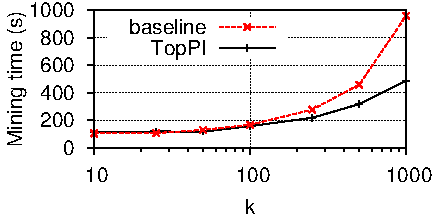
\includegraphics{fig/toppi/baseline/lastfm-s2-t16-timePerK.pdf}
			\caption{\em LastFM}
			\label{fig:baseline:TperK:lastfm}
		\end{subfigure}
		&
		\begin{subfigure}[b]{0.48\textwidth}
			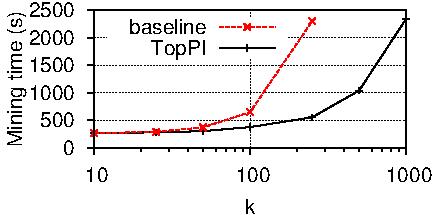
\includegraphics{fig/toppi/baseline/tickets2013-s2-t16-timePerK.pdf}
			\caption{\prodassocreceipt}
			\label{fig:baseline:TperK:prodassocreceipt}
		\end{subfigure}
		\\
		\begin{subfigure}[b]{0.48\textwidth}
			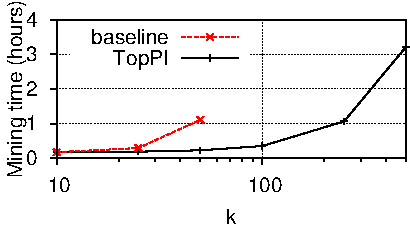
\includegraphics{fig/toppi/baseline/tickets2013-perClient-s2-t16-timePerK.pdf}
			\caption{\prodassocclient \\(11 hours at $k=1000$ for \toppi)}
			\label{fig:baseline:TperK:prodassocclient}
		\end{subfigure}
		&
		\hfill
		\begin{minipage}[b]{0.40\linewidth}
			\caption{\label{fig:baseline:TperK}
			\toppi and baseline run-times (in seconds), using 16 threads}
			\vspace{0.7in}
		\end{minipage}
		\\
	\end{tabular}
\end{figure}

Figure~\ref{fig:baseline:TperK} shows the run-times on our datasets when varying $k$,
not including the time necessary to load each dataset in memory.
Both solutions are equally fast for $k=10$, but as $k$ increases \toppi shows better performance.
The baseline even fails to terminate in some cases, either taking over 8 hours to complete, or running out of memory.
Instead \toppi can extract 50 CIS per item from \prodassocclient in 13 minutes,
or even 500 CIS per item out of the 320 million receipts of \prodassocreceipt in less than 20 minutes.

On \prodassocreceipt and \prodassocclient, the exponential increase of run-time
for $k \geq 200$ is explained by the increasing number of items having less than $k$ CIS.
In such cases, \toppi's mining becomes equivalent to frequent CIS mining with $\varepsilon = 2$.
In a discovery setting we only need 10 to 50 CIS per item so such complete exploration
of CIS branches only occur for rare items (having a support below 100 or 10, as shown p.~\pageref{fig:topKsize}),
where even a complete exploration is extremely fast.

{\em WebDocs} is missing in Figure~\ref{fig:baseline:TperK}:
even with 31 threads and $k=10$, \toppi takes 9.5 hours to complete.
In the same setting, the baseline completes the top-$k$ mining of only 3\% of the available items in 24 hours.
This is surprising, as in the frequent itemsets mining community {\em WebDocs} is always
classified as a sparse dataset, {\em ie.} it does not contain many frequent CIS.
But when running item-centric CIS mining, this is not the case:
\num{2242989} items occur in two transactions or more in {\em WebDocs}.
Some items also yield unusually large projected datasets,
typically a thousand transactions, each containing \num{20000} items (on average).
Such projected datasets are a worst case for both \toppi and its baseline,
which are optimized for datasets where transactions are much more numerous than items.
%Such an extreme distribution suggests that {\em WebDocs} does not fit our target use case,
%but is still useful for a load test for the {\em cluster} platform.


\begin{figure}
	\centering
	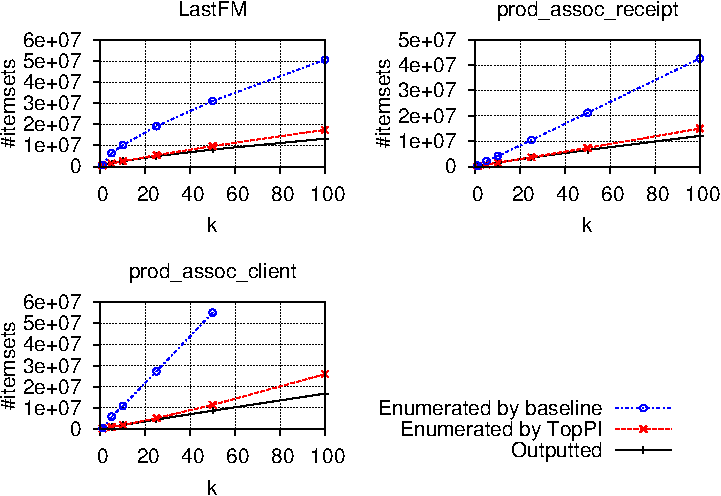
\includegraphics{fig/toppi/exploredVSoutputted/nbTraversed-perK-all.pdf}
	\caption{\label{fig:usefulVSexplored} Comparison of the number of itemsets
		explored by each algorithm with the number of itemsets actually outputted.
	}
\end{figure}

\begin{paragraph}{}
	To better understand the performance difference between \toppi and the baseline,
	we trace the execution of each algorithm to evaluate the number of itemsets enumerated.
	Figure~\ref{fig:usefulVSexplored} reports this result
	and compares it to the number of itemsets actually present in the output.
	Ideally, the algorithm should only enumerate outputted solutions.
	As explained in Section~\ref{sec:toppi:pruning},
	the problem of item-centric CIS mining is not anti-monotone,
	so both solutions have to enumerate a few additional itemsets to reach some solutions.
	Thanks to the the use of appropriate heuristics to guide the exploration,
	\toppi only enumerates a small fraction of discarded itemsets, which explains its good performance.
\end{paragraph}

Conversely, TFP enumerates a significant amount of itemsets that do not contribute to the output.
While it is highly efficient when mining the projected datasets of the most frequent items,
for the others TFP struggles to find the frequency threshold which guarantees
the correctness of its top-$k$.
When supports are counted in thousands, many more CIS have a similar support.
It also does not perform closure extensions,
but merges enumerated itemsets into their closure.
Hence its deeper traversal of the CIS space.

As each ${\cal D}[i]$ is mined independently for all items $i$,
the baseline cannot amortize the thresholds adaptations from a branch to another,
so this result would likely be also observed with another top-$k$ CIS mining algorithm.
This highlights the need for a specific algorithm for item-centric CIS mining.


\subsubsection{Scalability}

\begin{figure}
	\centering
	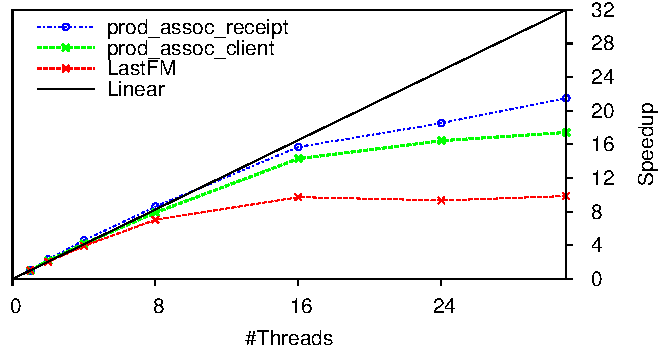
\includegraphics[]{fig/toppi/multithspeedup/all-mining.pdf}
	\caption{\label{fig:toppiSpeedup}\toppi speedup on {\em server} (with 16 physical cores and $k=50$)}
\end{figure}

We now evaluate how the centralized parallel version of \toppi leverages additional threads for the CIS exploration.
We report the mining time speedup with respect to the number of mining threads in Figure~\ref{fig:toppiSpeedup}.
%This measure uses up to 31 threads, leaving one core for the system.
As this machine has 16 physical cores, we cannot expect a perfect speedup with more than 16 threads.
We use up to 31 threads only;
because we only have 16 CPU cores (with hyper threading) this leaves the last virtual thread
to the system or the Java Virtual Machine's garbage collector.

Overall, \toppi achieves excellent scalability.
Depending on the size of the dataset, the limiting factor is either the CPU,
in which case adding more cores provides linear scalability (\prodassocreceipt and \prodassocclient),
or the memory bus, in which case the scalability is sub-linear above 8 threads (\emph{LastFM}).

\begin{figure}
	\centering
	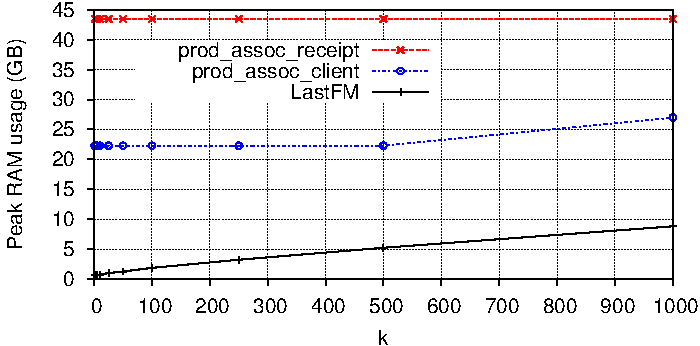
\includegraphics{fig/toppi/ram/RAM-all.pdf}
	\caption{\label{fig:ram}
		\toppi peak memory usage, using 31 threads
	}
\end{figure}

\begin{paragraph}{}
When 31 threads are used in parallel,
31 branches of the CIS tree are explored simultaneously and therefore held in memory,
with the corresponding stack of reduced datasets.
Though, even with 31 threads, the peak memory usage of \toppi remains reasonable.
This is confirmed by Figure~\ref{fig:ram},
where we report \toppi's peak RAM consumption  for \emph{LastFM}, \prodassocreceipt and \prodassocclient.
As expected, this peak increases with $k$.
Not only the top-$k$ collector is expanded accordingly,
but the $\mathit{prune}$ function also guides \toppi towards deeper tree explorations to generate additional itemsets,
thus keeping more reduced datasets in memory.
However this is less visible for \prodassocreceipt and \prodassocclient,
where the size of these objects is negligible compared to the initial dataset and its indexes.
\end{paragraph}

\begin{paragraph}{}
{\em WebDocs} is missing again in this study.
As \toppi takes 9.5 hours to complete with 31 threads and $k=10$,
we could not afford the memory study for $k \in [1, 1000]$,
nor the run-time measurement with a single thread.

Overall, these results confirm that \toppi is fast and scalable.
Even on common hardware:
\toppi is able to mine \textit{LastFM} with $k=50$ on a
laptop with 4 threads (Intel Core i7-3687U) and 6 GB of RAM in 16 minutes,
while this operation takes 13 minutes for PFP on our \textit{cluster} configuration with 200 cores,
as presented in the next section.
\end{paragraph}





\subsection{\toppi over Hadoop}
\label{sec:toppi:xp:hadoop}

Although the multi-threaded version of \toppi is able to mine millions of transactions
on a single server or even a laptop,
mining long tail itemsets from a more challenging dataset like \emph{WebDocs} requires more computational power.
A 25GB file like \prodassocreceipt and its memory requirement may also be out of reach of the analyst's machine
and, as in the \datalyse project, she may have a Hadoop cluster at hand instead of a single high-end server.
These examples motivated the development of the Hadoop variant of \toppi,
presented in Section~\ref{sec:toppi:distributed} and evaluated hereafter.

\subsubsection{Performance comparison to PFP}

\begin{figure}
	\centering
	\begin{subfigure}[b]{0.48\textwidth}
		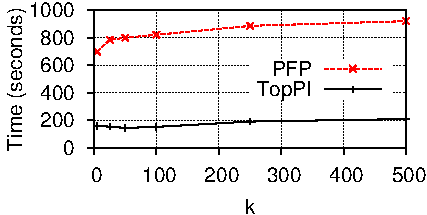
\includegraphics{fig/toppi/variousK/runtime-lastfm.pdf}
		\caption{\em LastFM}
	\end{subfigure}
	\hfill
	\begin{subfigure}[b]{0.48\textwidth}
		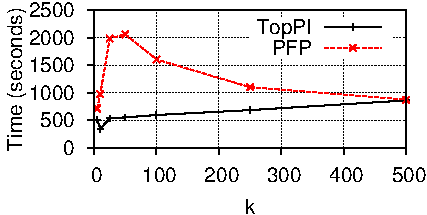
\includegraphics{fig/toppi/variousK/runtime-supermarket.pdf}
		\caption{\em Supermarket}
	\end{subfigure}
	\caption{\label{fig:PFP:runtime}
		\toppi and PFP run-times on a 200-tasks Hadoop cluster
	}
\end{figure}


In the following experiment we compare our Hadoop variant to PFP~\cite{LiRecSys08},
the closest algorithm to \toppi:
it returns, for each item, at most $k$ frequent itemsets containing that item.
We use the implementation\footnote{
Mahout 0.7 provides two implementations of PFP.
The alternative one is more memory-consuming, so for these experiments we
use the default implementation.
} available in the Apache Mahout Library~\cite{mahout}.
We use 50 worker machines and launch 4 tasks per machine, allocating 5GB of memory to each.
Hence, up to 200 MapReduce tasks are launched in parallel.
Even with this computing power at hand,
PFP is not able to mine \prodassocreceipt, \prodassocclient, nor {\em WebDocs}
--- even if we allocate more memory to mining tasks.
As only {\em LastFM} remains,
for this comparison we introduce a new dataset, \textit{Supermarket}, which is a preliminary version of \prodassocreceipt.
This 2.8GB file contains \num{54.8} million receipts
over \num{389372} items\footnote{That is almost twice as many products as in the final version.
A majority of products in this preliminary set are actually rare and unlabeled products,
which makes the qualitative study impractical. They have been removed in the final version.},
from 87 supermarkets over 27 months.
Its items distribution is very similar to \prodassocreceipt.

As PFP is not multi-threaded,
to ensure the fairness of the comparison
\toppi uses a single thread per task.
Mahout's documentation recommends to create one task for every 20 to 30 items,
thus PFP runs $\num{20000}$ tasks on \textit{LastFM}
%(\textit{LastFM} contains $\num{450399}$ items occurring at least 2 times),
%Figure~\ref{fig:topKvsKRuntimeLastFM} shows that
and $\num{17000}$ on \textit{Supermarket}.
\toppi launches 200 tasks.
%the execution time of \toppi and PFP when varying $k$.
The measured run-times are presented in Figure~\ref{fig:PFP:runtime}.

On \textit{LastFM},
increasing the value of $k$ has only a moderate influence on \toppi's run-time because,
when distributed among 200 tasks, the mining phases are very short
so the reported execution time mostly consists of Hadoop I/O.
\toppi remains 3 to 4 times faster that PFP.

On \textit{Supermarket}, PFP's run time is surprisingly uncorrelated to $k$.
PFP can also not terminate correctly above $k \geq 1000$ (\toppi can still run with $k \geq 2000$).
This may be caused by an implementation corner case,
or by the difference between the two algorithms' problem statements ---
\toppi provides stronger guarantees on long tail itemsets.


\subsubsection{Comparing PFP and \toppi's output}

\begin{figure}
	\centering
	\begin{subfigure}[b]{0.48\textwidth}
		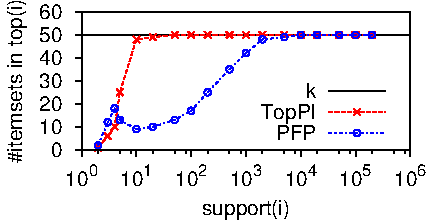
\includegraphics{fig/toppi/averagePatternsInTopKPerItem/lastfm-s2-k50.pdf}
		\caption{\em LastFM}
	\end{subfigure}
	\hfill
	\begin{subfigure}[b]{0.48\textwidth}
		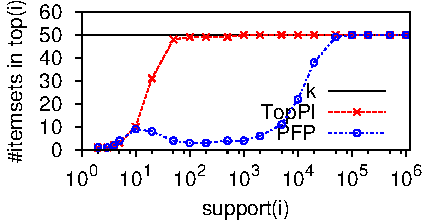
\includegraphics{fig/toppi/averagePatternsInTopKPerItem/supermarket-s2-k50.pdf}
		\caption{\em Supermarket}
	\end{subfigure}
	\caption{\label{fig:topKsize}
		Average $|\mathit{top}(i)|$ per item w.r.t. $\mathit{support}_{\cal D}(i)$ ($k=50$)
	}
\end{figure}



\toppi and PFP both rely on an item-centric approach and return,
for each frequent item $i \in {\cal I}$, at most $k$ frequent itemsets containing $i$.
But \toppi adds the guarantee that these $k$ itemsets are closed and the most frequent ones.
%We refer to Section~\ref{sec:rel:pfp} for more details on how PFP leverages the $k$ parameter.
We now compare the output of \toppi and PFP, using $k=50$,
to understand the impact
of these different problem statements on the results returned for long tail items.

Figure~\ref{fig:topKsize} shows the average number of itemsets outputted for each item,
with respect to its frequency.
In order to make these measures readable, we average them over item frequency intervals.
For the least frequent items, neither \toppi nor PFP manages to output the requested $k$ itemsets.
This is expected as an item of frequency 3, for example, can be part of at most 4 CIS.
For these items PFP returns more itemsets than \toppi on \textit{LastFM},
but most of them are redundant
--- both algorithms give the same number of {\em closed} itemsets.
As item frequency increases, \toppi returns more itemsets,
with almost  filled top-$k$ heaps for all items appearing at least 10 times in the dataset.
PFP, however, is unable to find these itemsets
and only returns close to $k$ itemsets for items whose frequency is above $\num{1000}$.
The difference is even more striking on \textit{Supermarket},
where PFP provides the required $k$ itemsets per item only for items occurring more than \num{10000} times.

This comes from PFP's division of the mining workload:
its mining phase fills a single top-$k$ heap per group of items.
%thus generating at most $k$ distinct itemsets per mining phase~\cite{LiRecSys08}.
%PFP instantiates a separate heap per item only in its last job and fills them using the results of the mining phase.
Thus, an item with a low frequency is unlikely to obtain $k$ itemsets as, during the mining,
itemsets corresponding to more frequent items of its group will fill the heap.
To mitigate this problem, Mahout's documentation recommends to raise the number of item groups,
such that each group only contains 20 to 25 items,
but this does not guarantees to obtain a complete top-$k$ per item.

These results show that, unlike PFP, \toppi performs a complete top-$k$ CIS mining for all items,
even long tail ones.%the ones with very low support, while PFP misses results for the long tail.

%These observations can be explained by analyzing each algorithm.
%\toppi maintains a distinct top-$k$ heap of results for each item throughout all the steps of the execution,
%to ensure that the results obtained are the precise top-$k$ CIS of the item.



\subsubsection{Scalability over Hadoop}

\begin{figure}
	\centering
	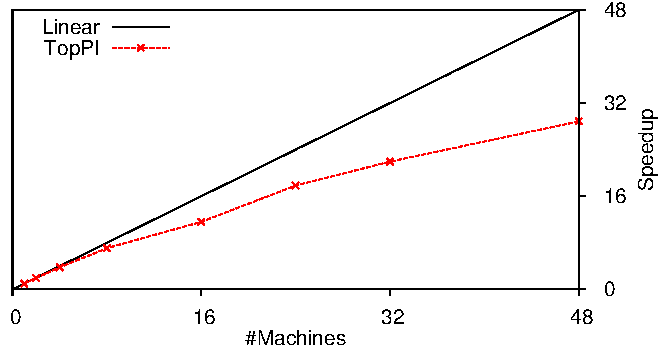
\includegraphics[]{fig/toppi/hadoop-speedup/supermarket-s2-k1000-t8.pdf}
	\caption{\label{fig:hadoopSpeedupGlobal}
		\toppi speedup when mining \textit{Supermarket} on Hadoop,
		using $k=1000$.
		Each machine is assigned a single items group and uses 8 threads.
	}
\end{figure}

Figure~\ref{fig:hadoopSpeedupGlobal} shows the speedup gained by the addition of worker nodes,
on \textit{Supermarket}, when $k=1000$.
Here we execute a single mining task per machine,
which fully exploits the available resources by running 8 threads in all the available memory, 24GB.

\toppi shows a perfect speedup from 1 to 8 machines (64 cores),
and steadily gets faster with the addition of workers.
Overall, the total CPU time (summed over all machines) spent in the mining phases ($\mathit{expand}$ function) remains stable:
from $\num{35000}$ seconds on average from 1 to 8 machines,
it only raises to $\num{38500}$ seconds with 48 machines (using their 384 cores).
Above, the speedup remains linear but below the ideal parallelization.
%Adding a task to \toppi incurs I/O costs, such as the time spent reading the initial dataset.
%Hence there is a trade-off between the execution time of the mining phases
%and the I/O overhead.
In this configuration, the sweet spot is around 8 tasks.
Should the workload increase,
\toppi would achieve optimal speedup on larger clusters,
as the overall mining time increases and compensates the I/O costs.
This is easily understandable,
as we selected parameters such that the experiment could also run on a single machine.
Above 16 tasks,
the I/O overhead represents a more significant fraction of the execution time and the efficiency decreases.

We further confirm \toppi's scalability by mining \emph{WebDocs} with $k=10$.
This computation takes \num{4570} seconds with 32 machines and \num{2641} with 64.
This represents a 1.7 speedup when doubling the tasks count.
This validates the distribution strategy used for the mining phases:
the load is well partitioned and does not increase significantly with the number of tasks.

\begin{figure}
	\centering
	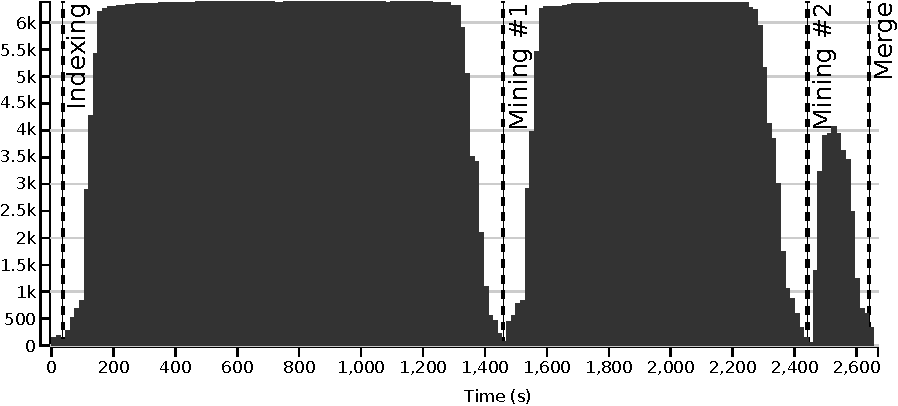
\includegraphics[]{fig/toppi/hadoopCpuLoad-webdocs-s2-k10-t8-g64-c.pdf}
	\caption{\label{fig:hadoopCpuLoad}
		\toppi aggregated CPU usage on a 64-machines cluster on \textit{WebDocs}
		($k=10$, 64 tasks running 8 threads each)
	}
\end{figure}

We confirm these observations by measuring the aggregated CPU usage of the whole cluster when using 64 workers.
The results are depicted on Figure~\ref{fig:hadoopCpuLoad}.
The mining phases correspond to high CPU usage, while I/O operations have low CPU usage.
As we can see, the amount of I/O is not negligible, which explains the lower speedup gain with 64 machines.
We also observe that the second mining phase is shorter than the first one.
Indeed, as described in Section~\ref{sec:toppi:distributed} (p.\pageref{sec:toppi:distributed}),
it leverages the per-item bounds discovered during the first stage.
While the first phase returns $\num{4037769}$ itemsets,
the second one returns significantly less ($\num{999511}$),
hence its shorter run-time.

The CPU usage distribution shows that both mining tasks complete on all servers in comparable amounts of time.
We do not observe straggler tasks significantly delaying \toppi.
Hence, \toppi balances well the load among the machines.












\section{Technology transfer}
\label{sec:toppi:integration}

As \toppi has been delivered early in the \datalyse project,
it benefited from the feedback of our industrial partners
who could run the program on the production cluster.
In this section, we summarize this feedback and its impact on our work.

\subsection{Run-time impact of sub-datasets instantiation}

The first results from industrial tests confirmed that \toppi is able to provide
%data to a receipts exploration application,
%which in turn is able to provide
insights on all the available products of a retailer as big as Intermach\'e.
However, sometimes the mining takes hours to complete.
Although the analytics cluster supporting these tests is small (4 workers with 4 CPU cores)
for datasets counting their size in gigabytes, such run-times are unexpectedly long.
Those are caused by the instantiation of sub-datasets,
which create many transactions duplicates.
This is discussed in Section~\ref{sec:subdatasets}.

We should also note that this transactions duplication is imposed by our search of {\em closed} itemsets.
Indeed we need complete transactions to perform the first-parent test (see Definition~\ref{def:firstparent}, p.\pageref{def:firstparent}).
Another way to run efficiently \toppi over MapReduce would be to relax this constraint,
thus allowing the transmission of truncated transactions as does PFP~\cite{LiRecSys08}.
Relaxing the constraint on closures would however include duplicate information
and decrease the results' quality.
Hence it can only be considered on extremely sparse datasets
(like {\em Supermarket} or \prodassocreceipt).
We also remark that these considerations also apply to distributed CIS mining:
our distribution of the exploration could as well be used with \jlcm.
It would even be simpler for \jlcm, which would only require the items indexation
and a single mining job ({\em cf.} Section~\ref{sec:toppi:hadoop}).

Overall, the Hadoop variant of \toppi is able to tackle all our datasets,
but the perfect speedup quest of distributed CIS mining would require a lot of ad-hoc development.
As analyzing a year worth of receipts is not done on a daily basis,
considering this run-time as acceptable is up to the analyst's patience and resources.
But the evolution of hardware suggests to keep such computations local:
mining the top-50 CIS per items from \prodassocreceipt takes 20 minutes on our experimental server
(including 15 minutes of dataset loading).



\subsection{The noise of star products}
\label{sec:toppi:stars}

The other important feedback about \toppi is qualitative.
Some of the most frequent products are orders of magnitude more frequent than others.
Marketing experts pay special attention to them, and nickname them ``star products''.
These include, for example, cola, shopping bags or grated cheese.
In \toppi's use case (dataset discovery) they are considered as noise:
because they are hyper-frequent, \toppi finds them combined with almost every other product,
hence showing one or more useless result(s) in those products' top-$k$.
For example, the association of most products with shopping bags does not provide any insight on
the product's associations ---
it only shows that customers often forget their shopping bag,
and have to buy the ones sold at the store.
We also observe this phenomenon in our {\em LastFM} dataset.
The most popular artists, like {\em The Beatles} or {\em Radiohead},
appear among the most frequent associations of almost all other artists (especially for large values of $k$).
Such results are artifacts of ``pop stars''.

As a workaround, for retail data our industrial partners filtered out star products
when curating transaction sets ({\em cf.} Section~\ref{sec:scenarios} p.\pageref{sec:scenarios}).
However, the list of star products is likely to evolve and will be difficult to maintain over the long-term
in the analytics system.
Also, there may be products having interesting associations with star products,
or on the other hand some products may appear as noise unexpectedly.

This shows the limits of ranking by frequency and
motivated our first experiments with the $p$-value, % (Section~\ref{sec:quali:pval})
and the development of \capa (Chapter~\ref{chap:capa}).
The second version of \toppi delivered to our industrial partners includes
a final re-ranking of itemsets in $\mathit{top}(i), \forall i \in \cal I$,
by decreasing correlation with the corresponding $i$.
We further discuss this method in Section~\ref{sec:quali:pval} (p.\pageref{sec:quali:pval}),
after studying alternative ranking functions in Chapter~\ref{chap:capa}.
% This requires a additional scan of $\cal D$.
% Indeed, while we have for each item $i$ a collection of CIS of the form $\{i\} \cup I$ (where $i \notin I$)
% and their supports, computing the $p$-value also requires $\mathit{support(I)}$ for each remainder $I$.
% This support search and re-ranking adds a few minutes to the execution over Hadoop,
% but provides a result set more adequate to \toppi's use case.


\section{Conclusion}
\label{sec:toppi:conc}

To the best of our knowledge,
\toppi is the first algorithm to formalize and solve at scale
the problem of mining item-centric top-$k$ closed itemsets,
a semantic more appropriate to early explorations of long-tailed datasets.
\toppi is able to operate efficiently on long tail content,
which is out of reach of standard mining and global top-$k$ algorithms.
Instead of generating millions of itemsets only containing the very few frequent items,
\toppi spreads its exploration evenly to mine a fixed number of $k$ itemsets for each item in the dataset,
including rare ones.
This is particularly important in the context of Web datasets,
in which the long tail contains most of the information~\cite{GoelWSDM10},
and in the retail industry, where it can account for a large fraction of the revenue~\cite{Anderson2006}.

\toppi scales from multi-cores to Hadoop clusters,
and is able to analyze a year of activity of \num{1884} Intermarch\'e stores in minutes on a single server,
allowing data analysts to easily obtain key associations for any product,
including very infrequent ones.
We demonstrate that \toppi's results are interesting by themselves,
but the following chapter suggests that \toppi can also be used as a building block to obtain alternative results
based on refined interestingness measures.% such as the $p$-value.
